\documentclass[../main.tex]{subfiles}

\begin{document}

\begin{customexercise}{5.3.2}
If $n\neq0$, the complex projective $n$-space $\mathbb CP^n$ is a simply connected manifold of dimension $2n$. As such $H_p(\mathbb CP^n)=0$ for $p>2n$. Given that there is a fibration $S^1\to S^{2n+1}\to\mathbb CP^n$, show that for $0\leq p\leq 2n$
\begin{align*}
H_p(\mathbb CP^n)\cong\begin{cases}
\mathbb Z &p\text{ even} \\
0 &p\text{ odd}
\end{cases}
\end{align*}
\end{customexercise}

\begin{proof}
The $E^2$ page looks like
\begin{center}
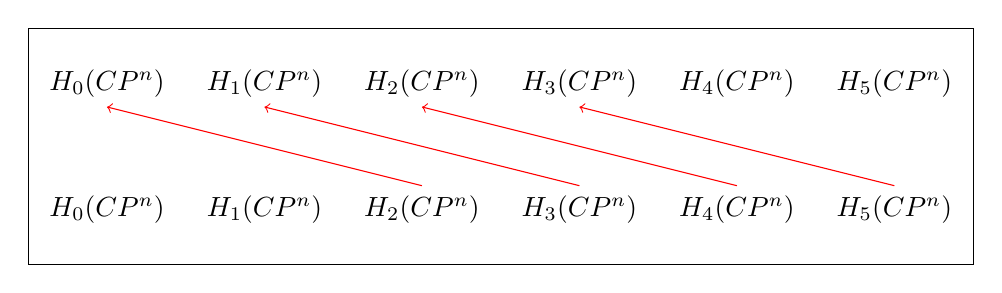
\begin{tikzpicture}
\draw (-1,-1)--(11,-1)--(11,2)--(-1,2)--cycle;
\foreach \x in {0,1,...,5}
{

\node at (2*\x,0)[below] {$H_{\x}(\mathbb CP^n)$};
\node at (2*\x,1)[above] {$H_{\x}(\mathbb CP^n)$};
}
\foreach \x in {2,...,5}
{
\draw[red,->] (2*\x,0)--(2*\x-4,1);
}
\end{tikzpicture}
\end{center}
Thus we have
\[E^\infty_{p1}=E^3_{p1}=\mathrm{coker}(H_{p+2}(\mathbb CP^n)\to H_{p}(\mathbb CP^n))\]
\[E^\infty_{p0}=E^3_{p0}=\begin{cases}
\ker(H_p(\mathbb CP^n)\to H_{p-2}(\mathbb CP^n)) &p\geq2 \\
0 &p=0,1
\end{cases}\]
\[\bigoplus_{p=0}^{k}E^3_{p,k-p}=\bigoplus_{p=0}^{k}E^\infty_{p,k-p}=H_k(S^{2n+1})=\begin{cases}
\mathbb Z &k=0,2n+1 \\
0 &\text{otherwise}
\end{cases}\]
Since $H_0(\mathbb CP^n)=\mathbb Z$ and $H_k(S^{2n+1})=0$ for $k=2,\cdots,2n$, we know $H_1(\mathbb CP^n)=0$ and $H_{k}(\mathbb CP^n)\to H_{k-2}(\mathbb CP^n)$ are isomorphisms for $k=2,\cdots,2n$, hence for $0\leq p\leq2n$
\begin{align*}
H_p(\mathbb CP^n)\cong\begin{cases}
\mathbb Z &p\text{ even} \\
0 &p\text{ odd}
\end{cases}
\end{align*}
\end{proof}

\begin{customexercise}{5.4.1}
Recall that the completion $\widehat C$ is a filtered complex. Show that $C/F_{p-k}C$ and $\widehat C/F_{p-k}\widehat C$ are naturally isomorphic
\end{customexercise}

\begin{proof}
Fix $p$, we have exact sequence
\[0\to F_pC/F_{p-k}C\to C/F_{p-k}C\to C/F_pC\to 0\]
Since $F_pC/F_{p-k}C$ satisfies Mittag-Leffler condition, take limit we get exact sequence
\[0\to F_p\widehat{C}\to\widehat C\to C/F_pC\to\varprojlim_k\textstyle^1{F_pC/F_{p-k}C}=0\]
Thus $C/F_pC$ is naturally isomorphic to the cokernel $\widehat C/F_p\widehat{C}$
\end{proof}

\begin{customexercise}{5.4.2}
Show that the spectral sequences for $C$, $\bigcup F_pC$, and $C/\bigcap F_pC$ are all isomorphic
\end{customexercise}

\begin{proof}
The spectral sequence of $C$ and $\bigcup F_pC$ are isomorphic since they define the same $A^r_p=\{c\in F_pC|dc\in F_{p-r}C\}$ thus the same $Z^r_p,B^r_p,E^r_p$ \par
The spectral sequence of $C$ and $C/\bigcap F_pC$ are isomorphic since $\displaystyle\varprojlim_k\dfrac{C/\bigcap F_pC}{F_kC/\bigcap F_pC}\cong\varprojlim_k C/F_kC$, i.e. they have the same completion
\end{proof}

\begin{customexercise}{5.4.3}(Shifting or D\'ecalage) Given a filtration $F$ on a chain complex $C$, define two new filtrations $\widetilde F$ and $\mathrm{Dec} F$ on $C$ by $\widetilde F_pC_n=F_{p-n}C_n$ and $(\mathrm{Dec}F)_pC_n=\{x\in F_{p+n}C_n|dx\in F_{p+n-1}C_{n-1}\}$. Show that the spectral sequences for these three filtrations are isomorphic after reindexing: $E^r_{pq}(F)\cong E^{r+1}_{2p+q,-p}(\widetilde F)$ for $r\geq0$, and $E^r_{pq}(F)\cong{} E^{r-1}_{-q,p+2q}(\mathrm{Dec} F)$ for $r\geq2$
\end{customexercise}

\begin{proof}
$E^r_{pq}(F)\cong E^{r+1}_{2p+q,-p}(\widetilde F)$ for $r\geq0$ since
\[\widetilde A^{r+1}_{2p+q,-p}=\left\{x\in\widetilde F_{2p+q}C_{p+q}\middle|dx\in\widetilde F_{2p+q-r-1}C_{p+q-1}\right\}=\left\{x\in F_{p}C_{p+q}\middle|dx\in\widetilde F_{p-r}C_{p+q-1}\right\}=A^r_{p,q}\]
\begin{align*}
(\mathrm{Dec}A)^{r-1}_{-q,p+2q}&=\left\{x\in (\mathrm{Dec}F)_{-q}C_{p+q}\middle|dx\in(\mathrm{Dec}F)_{-q-r+1}C_{p+q-1}\right\} \\
&=\left\{x\in F_pC_{p+q}\middle|dx\in F_{p-1}C_{p+q-1},dx\in F_{p-r}C_{p+q-1},0=d^2x\in F_{p-r-1}C_{p+q-2}\right\} \\
&=\left\{x\in F_pC_{p+q}\middle|dx\in F_{p-r}C_{p+q-1}\right\} \\
&= A^r_{p,q}
\end{align*}
\end{proof}

\end{document}